% -*- coding: utf-8; mode: latex; -*-

% +++
% latex = "lualatex"
% +++

%
% FIT2023 向け LaTeX クラスファイル
% https://github.com/trueroad/FITpaper-class
%
% サンプルファイル
%
% Copyright (C) 2018, 2019, 2022, 2023 Masamichi Hosoda.
% All rights reserved.
%

\documentclass{FITpaper}

% 図の貼り込み用
\usepackage{graphicx}

% 最終ページで両カラムの下端を揃える
%\usepackage[balance]{nidanfloat}
\usepackage{flushend}

% 和文タイトル
\jtitle{ブラウザ上でユーザが編集可能な言語パターンマッチシステムの構築 }

% 欧文タイトル
\etitle{Building a user-editable language pattern matching system in the browser}

% 著者数:著者の数だけ c を書く
\authors{cc}

% 和文著者名:著者名間に & を書く
% 所属番号を \affmark でつける
\jauthors{%
  桂 辰弥\affmark{1} &
  竹内 孔一\affmark{1}
}

% 欧文著者名:著者名間に & を書く
\eauthors{%
  Tatsuya Katsura &
  Koichi Takeuchi
}

% 所属
% \affmark でつけた番号毎に指定
\afftext{1}{岡山大学}


\begin{document}

\maketitle
\begin{abstract}
  テキスト中の特定の表現を見つけることは,言語および教育分野において必要となることがある.例えば語学学習において,言語を検索するのに用いるコンコーダンサがある.本研究ではユーザ自身が求める表現を検索ブロックで組み合わせてシステムに投入し,事例を検索できるシステムの開発を行っている.先行研究においてJavaScriptとPythonを利用した基本システムを構築したが,システムの本格利用にはいくつかの課題が残されている.そこで本報告では検索エンジンの中心部分であるPrologデータベースの実装の改良,および、大規模なテキストが扱えるためにデータベースをシステムに導入したので、この改良について報告する。 
\end{abstract}
\section{はじめに}
テキスト中の特定のフレーズや表現を見つけることは,言語および教育分野において必要となることがある.テキストデータから特定のキーワードやフレーズの出現位置や文脈を抽出するためのプログラムとしてコンコーダンサがある.コンコーダンサは語学学習において特定のフレーズや表現の使用例を実際の文脈で把握することで,語彙や文法の理解、単語の使用法や文脈の把握に役立ち,学習者の語彙や表現力の向上に役立つ.
例えば ではが提案している.

パターンマッチングはテキストの表層で検索を行う正規表現とは異なり,情報を抽出したい文を対象に予め関係する文や文の一部に対応する文構造のパターンを用意し,そのパターンに合致する結果を取得する.
本研究ではユーザ自身が求める表現を検索ブロックで組み合わせてシステムに投入し,事例を検索できるシステムの開発を行っている



先行研究においてWEBアプリケーションとしてJavaScriptとPythonを利用した基本システムを構築したが,
システムの本格利用にはいくつかの課題が残されている.そこで本報告では検索エンジンの中心部分であるPrologデータベースの実装の改良,および、大規模なテキストが扱えるためにデータベースをシステムに導入したので、この改良について報告する.
本研究の評価実験を行い,本システムでは10000文程度の比較的大きなコーパスを扱えることを確認できた.
\section{提案する言語パターンマッチシステム}
\subsection{言語パターンマッチシステムの概要}
\begin{figure}[htbp]
  \centering
  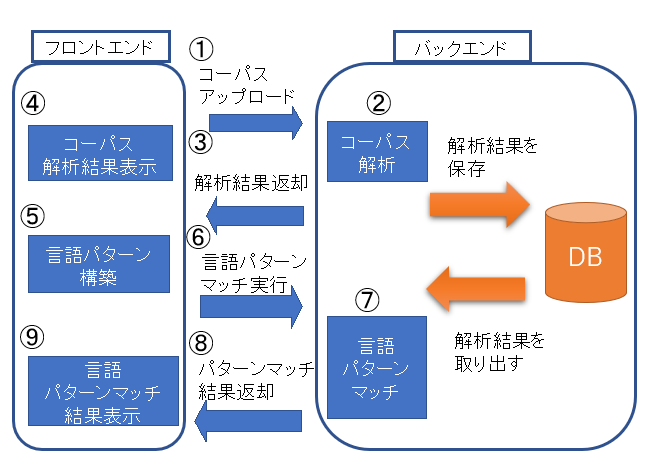
\includegraphics[scale=0.4]{fig/system_fig.png}
  \caption{システムの構成図}
  \label{fig:sys}
\end{figure}

\section{評価実験}


\acknowledgment{%
  謝辞の文章を\texttt{\textbackslash acknowledgment}で指定します。
  使わなければ謝辞は出力されません。
}

/%\bibliographystyle{unsrt}

%\bibliography{all,my-results}


\end{document}